\documentclass[11pt]{article}

\usepackage{extras} % Se extras.sty

\begin{document}
\begin{titlepage}
\begin{center}

{\Large\bfseries TSEA56 - Kandidatprojekt i elektronik \\ LIPS Teknisk dokumentation}

\vspace{5em}

Version 1.0

\vspace{5em}
Grupp 4 \\
\begin{tabular}{rl}
Hynén Ulfsjöö, Olle&\verb+ollul666+
\\
Wasteson, Emil&\verb+emiwa068+
\\
Tronje, Elena&\verb+eletr654+
\\
Gustafsson, Lovisa&\verb+lovgu777+
\\
Inge, Zimon&\verb+zimin415+
\\
Strömberg, Isak&\verb+isast763+
\\
\end{tabular}

\vspace{5em}
\today

\vspace{16em}
Status
\begin{longtable}{|l|l|l|} \hline

Granskad & - & - \\ \hline
Godkänd & - & - \\ \hline
 
\end{longtable}

\end{center}
\end{titlepage}

\pagebreak
\begin{center}

\section*{PROJEKTIDENTITET}
2016/VT, Undsättningsrobot Gr. 4

Linköpings tekniska högskola, ISY
\vspace{5em}
%\begin{center}

\begin{tabular}{|l|l|l|l|} \hline
\textbf{Namn} & \textbf{Ansvar} & \textbf{Telefon} & \textbf{E-post}  \\ \hline 
Isak Strömberg (IS) & Projektledare & 073-980 38 50 & isast763@student.liu.se \\ \hline
Olle Hynén Ulfsjöö (OHU)& Dokumentansvarig & 070-072 91 84 & ollul666@student.liu.se \\ \hline
Emil Wasteson (EW) & Hårdvaruansvarig & 076-836 61 66 & emiwa068@student.liu.se \\ \hline
Elena Tronje (ET) & Mjukvaruansvarig & 072-276 92 93 & eletr654@student.liu.se \\ \hline
Zimon Inge (ZI)& Testansvarig & 070-171 35 18 & zimin415@student.liu.se \\ \hline
Lovisa Gustafsson (LG) & Leveransansvarig & 070-210 32 53 & lovgu777@student.liu.se \\ \hline
\end{tabular}

%\end{center}

E-postlista för hela gruppen: isast763@student.liu.se

\vspace{5em}
Kund: ISY, Linköpings universitet 
tel: 013-28 10 00, fax: 013-13 92 82 \\
Kontaktperson hos kund: Mattias Krysander \\
tel: 013-28 21 98, e-post: matkr@isy.liu.se \\

\vspace{5em}
Kursansvarig:  Tomas Svensson\\
tel: 013-28 13 68, e-post: tomass@isy.liu.se \\
Handledare: Peter Johansson \\
tel: 013-28 13 45, e-post: peter.a.johansson@liu.se
\end{center}
\pagebreak

\tableofcontents

\pagebreak

\section*{Dokumenthistorik}
\begin{table}[h]
\begin{tabular}{|l|l|l|l|l|} \hline

\textbf{Version} & \textbf{Datum} & \textbf{Utförda förändringar} & \textbf{Utförda av} & \textbf{Granskad} \\ \hline
1.0 & - &  Första utkastet & Grupp 4 & - \\ \hline
\end{tabular}
\end{table}

\pagebreak
\pagenumbering{arabic}

\begin{flushleft}
\section{Inledning}
\textit{Bakgrund och syfte}

Projektets syfte är att konstruera en undsättningsrobot med kartläggning. Detta dokument syftar till att ge en detaljerad teknisk beskrivning av projektet på en nivå där resultatet ska kunna återskapas. Innehållet består av detaljerade beskrivningar av systemets olika delar, dess mjuk- och hårdvarukomponenter samt hur dessa är implementarade.

\section{Produkten}
\textit{En bild på produkten och en beskrivning av hur den fungerar. Beskriv vad den används till.}

Produkten som konstruerats är en undsättningsrobot. Den består av ett chassi, ett batteri, en av/på-brytare samt en gripklo. På chassit är huvudmodulen, sensormodulen och styrmodulen ihopkopplade med en I\textsuperscript{2}C-buss som sköter kommunikationen mellan dem. Roboten kommunicerar med datormodulen via Bluetooth\textsuperscript{\circledR}. Gripklon kontrolleras av styrmodulen och  det är sensormodulen som tar in data från sensorerna. För att montera sensorerna på chassit används 3D-printade fästen. En översiktlig bild av produkten återfinns i figur \ref{overview}.

Varje modul har en processor och övrig nödvändig hårdvara, som lågpassfilter och brytare, kopplade på ett virkort. Virkorten kan användas som grund för att tillverka kretskort med motsvarande funktion. 

Robotens uppgift är att söka av en labyrint bestående av 40 cm breda korridorer med hjälp av en avsökningsalgoritm och identifiera en nödställd som sänder ut IR-ljus. När målet är identifierat bestäms kortaste vägen mellan labyrintens ingång och målet. Efter det hämtar roboten en förnödenhet vid starten, kör kortaste vägen till den nödställda och lämnar av förnödenheten för att sedan ta sig tillbaka samma väg till starten. Utforskning och intern kartläggning av labyrinten sker simultant. Informationenen lagras för att kunna skickas vidare till datormodulen för uppritning. 


\begin{figure}[!htbp]
\centering
\noindent\resizebox{\linewidth}{!}{
	
\documentclass[border=10px]{standalone}
\usepackage{tikz}
\usetikzlibrary{patterns}
\usetikzlibrary{shapes.arrows}
\usepackage{amssymb}
\usetikzlibrary{calc}
\usepackage{verbatim}
\usetikzlibrary{decorations.pathmorphing}

\begin{document}
	
\begin{tikzpicture}[scale=1,rotate=0]
		
	%Base
	\draw[thick, draw=black, fill=gray!10] (0,0) rectangle (6,10);

	%Wheels
	\draw[thick, pattern=north west lines, pattern color=black] (-.5,1) 		rectangle (0,2.5);
	\draw[thick, pattern=north west lines, pattern color=black] (-.5,7.5) 	rectangle (0,9);
	\draw[thick, pattern=north west lines, pattern color=black] (6,1) 		rectangle (6.5,2.5);
	\draw[thick, pattern=north west lines, pattern color=black] (6,7.5) 		rectangle (6.5,9);
	
	%Sensors
	\draw[thick, draw=black, fill=white]		(-.25,.25) 		rectangle 	(.5,.75);
	\draw[thick, draw=black, fill=white] 	(-.25,9.25) 		rectangle 	(.5,9.75);
	\draw[thick, draw=black, fill=white] 	(5.5,.25) 		rectangle 	(6.25,.75);
	\draw[thick, draw=black, fill=white] 	(5.5,9.25) 		rectangle 	(6.25,9.75);
	\draw[thick, draw=black, fill=white] 	(1.5,10.25) 		rectangle 	(4.5,9.5);
	\draw[thick, draw=black]				 	(2.5,9.5)			--		  	(2.5,10.25);
	\draw[thick, draw=black]					(3.5,9.5) --++ (0,.75);
	
	%Gripklo
	\draw[thick, draw=black, <-] (3,10.25) --++ (0,.72) node[above] {Gripklo};
	
	%Lidar lite
	\draw[thick, draw=black, <-] 			(1.5,10.25)  		--+ 		  	(135:1) node[above, align=center] {\verb+LIDAR-Lite v2+ \\ med servo};
	%Identifierare av nödställd
	\draw[thick, draw=black, <-]				(4.5,10.25)		--+			(45:1)  node[above] {\verb+IRM-8601-S+};
	
	%IR sensorer
	\draw[thick, draw=black, <-]				(-.25, 9.75) 	--+			(135:1) node[above] {\verb+GP2D120+};
	\draw[thick, draw=black, <-]				(-.25, .25) 		--+			(225:1) node[below] {\verb+GP2D120+};
	\draw[thick, draw=black, <-]				(6.25, 9.75) 	--+			(45:1) node[above] {\verb+GP2D120+};
	\draw[thick, draw=black, <-]				(6.25, .25) 		--+			(315:1) node[below] {\verb+GP2D120+};
	
	\draw[thick, draw=black, fill=white]					(2.5,4.5)		rectangle	(3.5,5.5);
	
	%Gyro
	\draw[thick, draw=black, <-] (3.5,5) --++ (.25,0) node[rotate=270, above] {\verb+MLX90609+};
	
	%Arrows and text
	%\draw[thick, ->]  (3,11) node[left, align=center] {\verb+LIDAR-Lite v2+ \\ + detektor av nödställd} -- (3,10.25);
	%\draw[thick, <->] (0.5,0.5)  --  (5.5,0.5) node[left=-14pt,midway, fill=gray!10] {\verb+GP2D120+};
	%\draw[thick, <->] (0.5,9.5) -- (3,9) node[right=-14pt,fill=gray!10] {\verb+GP2D120+} -- (5.5,9.5);
	%\draw[thick, ->] (4.5,5) node[above] {\verb+MPU-6500+} -- (3.5,5);
	
	%Sensormodul
	\node (sensormodul) at (3,6.75) [thick, draw=black, minimum width=3cm, minimum height=1.5cm, align=center, fill=white] {Sensormodul \\ \verb+ATmega1284p+};
	
	%Huvudmodul
	\node (huvudmodul) at (3,3.25) [thick, draw=black, minimum width=3cm, minimum height=1.5cm, align=center, fill=white] {Huvudmodul \\ \verb+ATmega1284p+};
	
	%Styrmodul
	\node (styrmodul) at (3,1.25) [thick, draw=black, minimum width=3cm, minimum height=1.5cm, align=center, fill=white] {Styrmodul \\ \verb+ATmega1284p+};
	
	%I2C-buss
	\draw[thick, draw=teal] ($(sensormodul.north east) + (.25,0)$) -- ($(styrmodul.south east) + (.25,0)$);
	\draw[thick, draw=teal] ($(sensormodul.north east) + (.5,0)$) -- ($(styrmodul.south east) + (.5,0)$);
	\node (i2c) at ($(sensormodul.north east) + (0.375,.25)$) [text=teal] {\small I\textsuperscript{2}C};
	
	\draw[thick, draw=teal, fill=teal] ($(sensormodul.south east) + (0,.25)$) --+ (.25,0) circle [radius=.05cm];
	\draw[thick, draw=teal, fill=teal] ($(sensormodul.south east) + (0,.5)$) --+ (.5,0) circle [radius=.05cm];
	
	\draw[thick, draw=teal, fill=teal] ($(huvudmodul.south east) + (0,.25)$) --+ (.25,0) circle [radius=.05cm];
	\draw[thick, draw=teal, fill=teal] ($(huvudmodul.south east) + (0,.5)$) --+ (.5,0) circle [radius=.05cm];
	
	\draw[thick, draw=teal, fill=teal] ($(styrmodul.south east) + (0,.25)$) --+ (.25,0) circle [radius=.05cm];
	\draw[thick, draw=teal, fill=teal] ($(styrmodul.south east) + (0,.5)$) --+ (.5,0) circle [radius=.05cm];
	
	%Koppling till sensormodul
	\draw[thick, draw=violet] (.5,9.5) --++ (.25,0) --++ (0,-2.5) --++ (0.75,0) ;
	\draw[thick, draw=violet] (.5,.5) --++ (.25,0) --++ (0,6.25) --++ (0.75,0);
	
	\draw[thick, draw=violet] (5.5,9.5) --++ (-.25,0) --++ (0,-2.5) --++ (-0.75,0);
	\draw[thick, draw=violet] (5.5,.5) --++ (-.25,0) --++ (0,6.25) --++ (-0.75,0);
	
	\draw[thick, draw=violet] (2,9.5) --++ (0,-2);
	\draw[thick, draw=violet] (4,9.5) --++ (0,-2);
	
	\draw[thick, draw=violet] (sensormodul.south) --++ (0,-.5);
	
	%Kopplingar till styrmodul
	\draw[thick, draw=olive] (styrmodul.east) --++ (1.5,0);
	\draw[thick, draw=olive] (styrmodul.west) --++ (-1.5,0);
	\draw[thick, draw=olive] ($(styrmodul.east) + (0,.25)$) --++ (1,0) --++ (0,6.25) --++ (.5,0);
	\draw[thick, draw=olive] ($(styrmodul.west) + (0,.25)$) --++ (-1,0) --++ (0,6.25) --++ (-.5,0);
	\draw[thick, draw=olive] (3,9.5) --++ (0,-1.75) --++ (-1.75,0) --++ (0,-6) --++ (.25,0);
	
	%Bluetooth
	\draw[thick, draw=black] (huvudmodul.east) --++ (2,0) node[right,minimum width=.75cm, minimum height=1cm, draw=black] (bt) {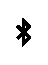
\includegraphics{bluetooth}};
	
	\node (bt2) at ($(bt) + (2,0)$) [thick, draw=black, minimum width=.75cm, minimum height=1cm] {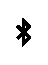
\includegraphics{bluetooth}};
	
	\draw[thick, ->,line join=round,decorate, decoration={
    												snake,
    												segment length=5,
    												amplitude=1,
    												post=lineto,
    												post length=1pt}] 
    		($(bt.east) + (5pt,5pt)$) -- ($(bt2.west) + (-5pt,5pt)$);
    		
    \draw[thick, ->,line join=round,decorate, decoration={
    												snake,
    												segment length=5,
    												amplitude=1,
    												post=lineto,
    												post length=1pt}] 
    		 ($(bt2.west) + (-5pt,-5pt)$) -- ($(bt.east) + (5pt,-5pt)$);
    		 
    \draw[thick, draw=black] (bt2.east) --++ (.5,0) node[right, minimum width=3cm, minimum height=1.5cm, draw=black, fill=white] {Datormodul};
    
    \draw[thick, draw=black] ($(sensormodul.south west) + (.25,0)$) --++ (0,-2) node[midway, above, sloped] {\small avbrott};
    
    \draw[thick, draw=black] ($(styrmodul.north west) + (.25,0)$) -- ($(huvudmodul.south west) + (.25,0)$) node[right, midway] {\small avbrott};
	
	\end{tikzpicture}
	
\end{document}  
}
	\caption{Det totala systemet \label{overview}}	
\end{figure}

\pagebreak

\section{Teori}
\textit{Beskrivning av regleralgoritmer mm.}

\subsection{Labyrintnavigering}
Nedan beskrivs principer för avsökning och kartläggning av labyrinter.

\subsubsection{Väggföljare}
Ifall labyrinten är enkelt sammanhängande räcker en väggföljar-algoritm för att kartlägga alla korridorer. I en enkelt sammanhängande labyrint är alla väggar kopplade till varandra, se figur \ref{maze} för exempel. En väggföljar-algoritm är antingen av höger- eller vänstertyp och bygger på att en av korriodens sidor alltid följs. Ifall algoritmen är av högertyp följs höger sida av korridoren och svänger höger där det är möjligt, vice versa för vänstertyp.

\begin{figure}[htbp]
	\centering
	\begin{subfigure}{.5\linewidth}
		\centering
		\noindent\resizebox{.5\textwidth}{!}{
			\documentclass[border=10px]{standalone}
\usepackage{tikz}
\usetikzlibrary{patterns}
\usetikzlibrary{shapes.arrows}
\usepackage{amssymb}
\usetikzlibrary{calc}
\usepackage{verbatim}
\begin{document}
	
\begin{tikzpicture}[scale=1]
		
		
		\draw[thick, ,draw=none, pattern=north west lines, pattern color=green] (1,1) rectangle (2,2);
		\draw[thick] (0,0) -- (0,4) -- (4,4) -- (4,0) -- (1,0);
		\draw[thick] (1,3) -- (1,1) -- (3,1) -- (3,3) -- (2,3);
		\draw[thick] (1,2) -- (2,2);
		
		\draw[thick, ->] (.5,-.5) -- (.5,-0);
		
		\draw[thick, ->,loosely dotted, draw=blue] (.2,0) -- (.2,3.8) -- (3.8,3.8) -- (3.8,.2) -- (1,.2);
		
	\end{tikzpicture}
\end{document}}
		\caption{En inte enkelt sammanhängande labyrint}	
		\label{non-connected}
	\end{subfigure}%
	\begin{subfigure}{.5\linewidth}
		\centering
		\noindent\resizebox{.5\textwidth}{!}{
			\documentclass[border=10px]{standalone}
\usepackage{tikz}
\usetikzlibrary{patterns}
\usetikzlibrary{shapes.arrows}
\usepackage{amssymb}
\usetikzlibrary{calc}
\usepackage{verbatim}
\begin{document}
	
\begin{tikzpicture}[scale=1]
		
		
		\draw[thick, ,draw=none, pattern=north west lines, pattern color=green] (1,1) rectangle (2,2);
		\draw[thick] (0,0) -- (0,4) -- (4,4) -- (4,0) -- (1,0);
		\draw[thick] (1,3) -- (1,1) -- (3,1) -- (3,3) -- (2,3);
		\draw[thick] (1,2) -- (2,2);
		\draw[thick] (3,1) -- (4,1);
		
		\draw[thick, ->] (.5,-.5) -- (.5,-0);
		
		\draw[thick, ->, loosely dotted, draw=blue] (.2,0) -- (.2,3.8) -- (3.8,3.8) -- (3.8,1.2) -- (3.2,1.2) -- (3.2,3.2) -- (1.8,3.2) -- (1.8,2.8) -- (2.8,2.8) -- (2.8,1.2) -- (2,1.2);
		
	\end{tikzpicture}
\end{document}}
		\caption{En enkelt sammanhängande labyrint}	
	\end{subfigure}%
	\caption{Exempel på labyrint och rutt som skulle tas av en väggföljningsalgoritm av vänstertyp}
	\label{maze}
\end{figure}%

Fördelar med algoritmen är att den är enkel att implementera men avsaknaden av intelligens gör att utforskandet av labyrinten tar lång tid. Algoritmen klarar endast att utforska de allra enklaste typer av labyrinter och ifall labyrinten inte är enkelt sammanhängande kan roboten fastna i en oändlig loop.

\subsubsection{\emph{Dead-end filling}}
\emph{Dead-end filling} är en djup-först-algoritm som utforskar en väg tills en återvändsgränd upptäcks. Därefter åker roboten tillbaka till den första korsningen som har outforskade utgångar och kartlägger dessa tills en ny återvändsgränd upptäcks. Denna process återupprepas tills hela labyrinten är kartlagd.

\subsection{Beräkning av kortaste väg}
Nedan beskrivs två algoritmer för att ta fram kortaste väg.

\subsubsection{Dijkstras algoritm}
Dijkstras algoritm är en girig, bäst-först-algoritm. Algoritmen beräknar den billigaste (kortaste) vägen från startnoden till samtliga noder och fungerar på nätverk med icke-negativa bågkostnader. 

Vid starten definieras två mängder, en med de avsökta och en med de oavsökta noderna. De oavsökta noderna har ett oändligt nodpris och startnoden har nodpriset noll. Med ursprung i startnoden söker algoritmen igenom alla grannar. Nodpriset updateras i det fall då följande samband gäller:

\begin{displaymath}
	y_i + c_{i,j} < y_j
\end{displaymath}

där \begin{math} y_i \end{math} är den nod som söks av, \begin{math} y_j \end{math} är nodgrannen och \begin{math} c_{i,j} \end{math} är kostnaden mellan nod \begin{math} i \end{math} och \begin{math} j \end{math}.

Ovanstående görs successivt med ursprung i den nod med billigast nodpris tills slutnoden har undersökts. Den kortaste vägen kan sedan nästlas upp, förutsatt att den föregångare noden som bidrog till en kortare väg sparas. 

En vidareutveckling av Dijkstras algoritm är A* som, med hjälp av en heuristik, väljer vilka noder som ska avsökas vidare.

\subsubsection{A*}
A* är ytterligare en bäst-först-algoritm med målet att finna den billigaste vägen mellan två noder. I grund och botten finns samma maskineri som i Dijkstras algoritm, med skillnaden att noder avsöks i stigande ordning enligt
\begin{equation*}
	f(n) = g(n) + h(n)
\end{equation*}
där $g(n)$ utgör kostnaden av rutten från startnod till nod $n$ och $h(n)$ en heuristik som estimerar den billigaste vägen från nod $n$ till slutnod. Med andra ord är Dijkstras algoritm ett speciallfall av A* där $h(n) = 0$.

$h(n)$ kan ses som en straffunktion som avtar nära slutnoden. A* kan alltså, till skillnad från Dijkstras algoritm, se framåt i nätverket och kan därför ta bättre beslut om vilka noder som ska uppdateras.

\subsection{Reglering}\label{subsection:reglering}
Roboten har två olika reglermoder: reglering av rotation och reglering av rak körning. Regleringen av rak körning har i sin tur fyra olika lägen, som anpassar vilken insignal som används i regleringen: inga väggar, vägg på vänster sida, vägg på höger sida och vägg på båda sidor.

Rotationen regleras genom öppen reglering. Robotens gyro ger en vinkelhastighet som sedan integreras (summeras) tills summan nått ett förutbestämt värde, varefter rotationen avbryts.

Reglering av rak körning innebär reglering av två utsignaler: robotens avstånd till framförvarande vägg och robotens avstånd till väggen/väggarna i korridoren. Avståndet till framförvarande vägg $s$ regleras i förhållande till det önskade avståndet $s^0$ genom reglering av hastigheten $v$ enligt följande ekvation
\begin{equation*}
	v = 
	\begin{cases}
		v_{pref} \qquad\qquad \forall \ (s - s^0) > 20 \\
		0.6 \cdot v_{pref} \qquad \forall \ 20 \geq (s - s^0) > 0 \\
		0 \qquad\qquad\qquad \forall \ (s - s^0)\leq 0 \\
	\end{cases}
\end{equation*}
där $v_{pref}$ är den användardefinierade maxhastigheten.

Avståndet till väggen regleras genom att beräkna önskad skillnad i hastighet mellan höger och vänster hjulpar $\Delta v$ utifrån främre avståndssensor $d_1$, bakre avståndssensorn $d_2$ och det önskade avståndet $d^0$ enligt följande ekvation
\begin{equation*}
	\Delta v = K \Bigg( P \Big( \frac {d_1 + d_2} {2} - d^0 \Big) + D (d_1 - d_2) \Bigg)
\end{equation*}
där $K, P, D > 0$ är konstanter som används för att justera regleringen. Beroende på vilka väggar som finns inom sensorernas räckvidd används antingen vänster eller höger avståndssensorer som insignal. Vid vänster vägg eller dubbla väggar används vänster och vid höger vägg används höger. Vid dubbla väggar anväds dock sensorerna på båda sidor för att bestämma  $d^0$ enligt
\begin{equation*}
	d^0 = \frac {d_{1,v} + d_{2,v} + d_{1,h} + d_{2,h}} {4}
\end{equation*}

Känner avståndssensorerna inte av väggar på någon sida kan inte avståndet till väggarna regleras och $\Delta v = 0$.

\section{Systemet}
\textit{Ett översiktligt blockschema och en beskrivning av hela systemet.}

Roboten i sin miljö finns illustrerad i figur \ref{system}. Den kan både köras manuellt och autonomt, något som bestäms av en brytare på roboten. Kommunikationen med datormodulen är dubbelriktad via Bluetooth\textsuperscript{\circledR}. Roboten ska klara sitt uppdrag utan kommunikation med datormodulen, det vill säga att kartläggning, styrning och optimering av kortaste väg sker lokalt hos roboten. Banan är uppbyggd enligt banspecifikationen och uppdraget utförs enligt tävlingsreglerna, se appendix [??].

\begin{figure}[htbp]
\centering
\noindent\resizebox{.8\linewidth}{!}{
	\documentclass[border=10px]{standalone}
\usepackage{tikz}
\usetikzlibrary{patterns}
\usetikzlibrary{shapes.arrows}
\usepackage{amssymb}
\begin{document}
	
\begin{tikzpicture}[scale=1]
		
		\draw[thick] 	(0,0) -- (0,3);
		\draw[thick] 	(1,7) -- (6,7) -- (6,2);
					
		\draw[thick,pattern=north west lines, pattern color=black]	 	(4,0) -- (4,2) -- (6,2) -- (6,0) -- (4,0);
		
		\draw[thick,pattern=north west lines, pattern color=black]
						(0,3) -- (3,3) -- (3,4) -- (1,4)
					--	(1,7) -- (0,7) -- (0,3);
		
		\draw[thick,pattern=north west lines, pattern color=black]
						(2,5) -- (3,5) -- (3,6) -- (2,6)
					--	(2,5);
					
		\draw[thick,pattern=north west lines, pattern color=black]		(4,3) -- (5,3) -- (5,6) -- (4,6)
					--	(4,3);
					
		\draw[thick,pattern=north west lines, pattern color=black]
				(4,0) -- (1,0) -- (1,2) -- (3,2) -- (3,0);
				
		\draw[thick,->] (0.5,0) -- (0.5,0.5);
		
		\draw[thick] (4.2,2.2) rectangle (5,2.8) node[pos=.5] {\tiny Robot};
		\draw[thick] (1.2,6.2) rectangle (1.8,6.8);
		\draw[thick,<-] (1.8,6.5) -- (2.3,6.5) node[right] {\tiny Nödställd};
		\draw[thick, <-,overlay] (5.1,2.5) [out=0,in=-45] to (7,4) node [right=.5em] {\tiny Bluetooth\textsuperscript{\circledR}};
		\draw[thick,->,overlay] (7,4) [out=125,in=180] to (9,5) ;
		\node[]  at (10,5) {
\includegraphics[scale=0.8]{laptop}};
		\node[overlay] at (10,4) {Datormodul};
	\end{tikzpicture}
	
\end{document}}
	\caption{Översikt av banan\label{system}}	
\end{figure}

\subsection{Beskrivning av systemet}
Roboten navigerar med hjälp av värden som fås från sensormodulens sensorer. En lasersensor som är fäst på ett servo mäter avstånd framåt, fyra IR-sensorer mäter robotens avstånd till sidoväggarna, ett gyroskop mäter robotens vinkelhastighet och en IR-detektor identifierar den nödställde. Med jämnna intervall kommunicerar sensormodulen dessa värden till huvudmodulen som i sin tur vidarebefordrar dem till styrmodulen. 

I styrmodulen är en regleringsmodell implementerad, vilken säkerställer att roboten färdas i mitten av korridorerna samt kan rotera både 90 och 180 grader utan att stöta emot väggar. Önskade värden kan skrivas ut på en LCD-display, vilken också är en del av styrmodulen.

Under färden sker autonom kartläggning och beräkning av kortaste väg mellan ingången och den nödställde. När roboten är uppkopplad mot datormodulen ritar mjukvaran på datorn successivt upp en karta och presenterar utvalda mätvärden i realtid. 

När den kortaste vägen är funnen använder roboten denna rutt för att förse den nödställde med en förnödenhet. Förnödenheten transporteras med hjälp av robotens gripklo som kontrolleras av styrmodulen.

På systemnivå är det om målet är funnet och om kortaste väg kan garanterats som avgör robotens beslut, vilket illustreras i figur \ref{blockSystem}.

\begin{figure}[htbp]
\centering
\noindent\resizebox{1\linewidth}{!}{
	\documentclass[border=10px]{standalone}
\usepackage{tikz}
\usetikzlibrary{patterns}
\usetikzlibrary{shapes.geometric}
\usetikzlibrary{shapes.arrows}
\usepackage{amssymb}
\usetikzlibrary{calc}
\usepackage{verbatim}

\pagestyle{empty}
\begin{document}

\tikzstyle{decision} = [diamond, draw,
    text width=4em, text badly centered, node distance=3cm, inner sep=0pt]
    
\tikzstyle{block} = [rectangle, draw,
    text width=5em, text centered, rounded corners, minimum height=4em]
	
\begin{tikzpicture}[scale=1]

%http://www.texample.net/tikz/examples/simple-flow-chart/

\node[block](start){Start};
\node[decision, below of = start, aspect = 2, text width = 8 em] (foundTarget) {Målet funnet?};
\node[block, below of = foundTarget, node distance = 3cm, text width = 7em] (explore) {Utforska enligt högerföljning};
\node[decision, right of = foundTarget, text width = 6em, aspect = 2, node distance = 6cm] (foundShortestPath) {Garanterat funnit kortaste väg?};
\node[block, below of = foundShortestPath, node distance = 3cm, text width = 7em] (exploreTargetFound) {Utforska enligt högerföljning och optimering};
\node[block, right of = foundShortestPath, node distance = 5cm] (pickUp) {Hämta förnödenhet vid start};
\node[block, right of = pickUp, node distance = 3cm, text width = 6em] (shortestPath) {Från start följa kortaste väg till målet};
\node[block, right of = shortestPath, node distance = 3cm] (drop) {Lämna förnödenhet};
\node[block, below of = drop, node distance = 3cm, text width = 7em] (return) {Återvänd till startpunkt den kortaste vägen};
\node[block, below of = return, node distance = 3cm] (stop) {Slut};

\draw[->](start) --  (foundTarget);
\draw[->](foundTarget) -- node[near start, right]{nej} (explore);
\draw[->] (explore.west) -| ++(-1,3) -| (foundTarget.west);
\draw[->](foundTarget) -- coordinate[midway] (aux) node[near start, above]{ja} (foundShortestPath);
\draw[->] (foundShortestPath) -- node[near start, right]{nej}(exploreTargetFound);
\draw[->] (exploreTargetFound) -| (aux);
\draw[->] (foundShortestPath) -- node[near start, above]{ja}(pickUp);
\draw[->] (pickUp) -- (shortestPath);
\draw[->] (shortestPath) -- (drop);
\draw[->] (drop) -- (return);
\draw[->] (return) -- (stop);

	\end{tikzpicture}
	
\end{document}}
	\caption{Övergripande blockschema för systemet}	\label{blockSystem}
\end{figure}

\section{Begränsningar}
Roboten är begränsad till att navigera i korridorer och kräver att alla korsningar består av 90-gradersvinklar.

\section{Modulerna}
\textit{Innehåller mera detaljerade blockschemor och beskrivningar av varje modul. Tänk på läsbarheten och växla mellan figurer och text.}

\subsection{Huvudmodulen}
I detta avsnitt följer en detaljerad beskrivning av systemets ingående moduler. 

\subsubsection{Mjukvara}
\begin{description}[style=unboxed, leftmargin=0cm]
  \item[huvudMain.c] som innehåller \textit{main}-funktionen, I\textsuperscript{2}C-kommunikationen och Bluetooth\textsuperscript{\circledR}-kommunikationen . I huvudloopen är det endast styrläge som uppdateras.
  \item[bluetooth.h] som är ett paket för Bluetooth\textsuperscript{\circledR}-kommunikationen.
  \item[I2C\_master.h] som är ett paket för masterenheten på I\textsuperscript{2}C-bussen.
  \item[searchPath.h] är ett paket som hanterar avsökning, kartläggning och beräkning av kortaste väg.
\end{description}


\subsubsection{Övergripande beskrivning}

Huvudmodulen har som uppgift att ta emot och förmedla information mellan de andra modulera, hantera den interna kartläggnigen samt att ta alla övergripande beslut. Bluetooth\textsuperscript{\circledR} används för att kommunicera med datormodulen och en avbrottsstyrd I\textsuperscript{2}C-buss används för att kommunicera med sensor- och styrmodulen, vilket visas i figur \ref{communication}. När det kommer till prioriteringen av sensor- och styrmodul har styrmodulen kopplats till en extern avbrottsingång med högre prioritet än sensormodulen.
=======
Huvudmodulen har som uppgift att ta emot och förmedla information mellan de andra modulera, hantera den interna kartläggnigen samt att ta alla övergripande beslut. Bluetooth\textsuperscript{\circledR} används för att kommunicera med datormodulen och en avbrottsstyrd I\textsuperscript{2}C-buss används för att kommunicera med sensor- och styrmodulen, vilket visas i figur \ref{communication}. Vad gäller prioritering av sensor- och styrmodul har styrmodulen kopplats till en extern avbrottsingång med högre prioritet än sensormodulen.

\begin{figure}[htbp]
\noindent\resizebox{.97\textwidth}{!}{
	\documentclass[border=20pt]{standalone}
\usepackage{tikz}
\usetikzlibrary{positioning}
\usetikzlibrary{calc}
\usetikzlibrary{decorations.pathmorphing}
\usepackage{amssymb}
\usetikzlibrary{shapes,arrows}

\begin{document}
	\begin{tikzpicture}[scale=1]
		
		\tikzset{every node/.style={thick, draw=black, align=center, minimum height=40pt, text width=100pt, minimum width=100pt}}
		\node(datormodul) {Datormodul};
		\node[right=10pt of datormodul,minimum height=20pt, minimum width=10pt,text width=10pt] (bt1) {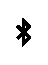
\includegraphics{bluetooth}};
		
		\node[right=40pt of bt1,minimum height=20pt, minimum width=10pt,text width=10pt] (bt2) {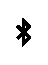
\includegraphics{bluetooth}};
		
		\node[right=10pt of bt2] 			(huvudmodul) 	{Huvudmodul};
		\node[below=-10pt of huvudmodul,draw=none] (master) {\textit{master}};
		\node[right=10pt of huvudmodul] 		(sensormodul) 	{Sensormodul};
		\node[below=-10pt of sensormodul,draw=none] (slave1) {\textit{slav}};
		\node[right=10pt of sensormodul] 	(styrmodul) 		{Styrmodul};
		\node[below=-10pt of styrmodul,draw=none] (slave2) {\textit{slav}};
		
		\coordinate (sclStart) 	at ($(huvudmodul.north west) + (0,20pt)$);
		\coordinate (sclEnd)		at ($(styrmodul.north east)  + (0,20pt)$);
		
		\coordinate (sdaStart)  at ($(sclStart) + (0,20pt)$);
		\coordinate (sdaEnd)		at ($(sclEnd)	+ (0,20pt)$);
		
		\coordinate (vddStart)  at ($(sdaStart) + (0,40pt)$);
		\coordinate (vddEnd)		at ($(sdaEnd)	+ (0,40pt)$);
		
		\draw[thick] (sclStart) -- (sclEnd) node [right,draw=none,text width=0,minimum width=0] {SCL};
		\draw[thick] (sdaStart) -- (sdaEnd) node [right,draw=none,text width=0,minimum width=0] {SDA};
		\draw[thick] (vddStart) -- (vddEnd) node [right,draw=none,text width=0,minimum width=0] {$V_{dd}$};
		
		\draw[thick] (datormodul.east) -- (bt1.west);
		
		\draw[thick, ->,line join=round,decorate, decoration={
    												snake,
    												segment length=5,
    												amplitude=1,
    												post=lineto,
    												post length=1pt}] 
    		($(bt1.east) + (5pt,5pt)$) -- ($(bt2.west) + (-5pt,5pt)$);
    		
    	\draw[thick, ->,line join=round,decorate, decoration={
    												snake,
    												segment length=5,
    												amplitude=1,
    												post=lineto,
    												post length=1pt}] 
    		 ($(bt2.west) + (-5pt,-5pt)$) -- ($(bt1.east) + (5pt,-5pt)$);
    		 
    	\draw[thick] (bt2.east) -- (huvudmodul.west);
    	
    	\draw[thick,fill=black] ($(huvudmodul.north) + (-10pt,0)$) -- ($(huvudmodul.north) + (-10pt,20pt)$) circle [radius=2pt];
    	\draw[thick,fill=black] ($(huvudmodul.north) + (+10pt,0)$) -- ($(huvudmodul.north) + (+10pt,40pt)$) circle [radius=2pt];
    	
    	\draw[thick,fill=black] ($(sensormodul.north) + (-10pt,0)$) -- ($(sensormodul.north) + (-10pt,20pt)$) circle [radius=2pt];
    	\draw[thick,fill=black] ($(sensormodul.north) + (+10pt,0)$) -- ($(sensormodul.north) + (+10pt,40pt)$) circle [radius=2pt];
    	
    	\draw[thick,fill=black] ($(styrmodul.north) + (-10pt,0)$) -- ($(styrmodul.north) + (-10pt,20pt)$) circle [radius=2pt];
    	\draw[thick,fill=black] ($(styrmodul.north) + (+10pt,0)$) -- ($(styrmodul.north) + (+10pt,40pt)$) circle [radius=2pt];
    	
    	\draw[thick,fill=black] ($(sensormodul.north east) + (-5pt,20pt)$) circle [radius=2pt] -- ($(sensormodul.north east) + (-5pt,80pt)$) circle [radius=2pt];
    	\draw[thick,fill=black] ($(styrmodul.north west) + (5pt,40pt)$) circle [radius=2pt] -- ($(styrmodul.north west) + (5pt,80pt)$) circle [radius=2pt];
    	\draw[thick,draw=black,fill=white] ($(styrmodul.north west) + (2pt,50pt)$) rectangle ($(styrmodul.north west) + (8pt,70pt)$);
		\draw[thick,draw=black,fill=white] ($(sensormodul.north east) + (-8pt,50pt)$) rectangle ($(sensormodul.north east) + (-2pt,70pt)$) node [below left=-10pt and 20pt,draw=none,minimum width=0, text width = 0pt] {$R_p$};
		
		\draw[thick, ->] ($(sensormodul.south) + (+40pt,0)$) -- ($(sensormodul.south) + (40pt,-30pt)$) -- ($(huvudmodul.south) + (40pt,-30pt)$) -- ($(huvudmodul.south) + (40pt,0)$);
		\draw[thick, ->] ($(styrmodul.south) + (+40pt,0)$) -- ($(styrmodul.south) + (40pt,-40pt)$) -- node [midway,below,minimum height=20pt, draw=none] {Avbrott}($(huvudmodul.south) + (30pt,-40pt)$) -- ($(huvudmodul.south) + (30pt,0)$);
	\end{tikzpicture}
\end{document}}
	\caption{Intermodulär kommunikation \label{communication}}
\end{figure}

\subsubsection{Styrlägen}
Det finns två olika körlägen för roboten, ett autonomt och ett manuellt läge. Rent hårdvarumässigt styrs val av läge med hjälp av en brytare kopplad till huvudmodulen. När det autonoma läget är aktiverat tas körbeslut utifrån en avsökningsalgoritm som i grunden använder sig av väggföljning av högertyp. Beslutet om vilken kartmodul som ska besökas härnäst baseras på datan som skickats från sensormodulen och på den interna kartläggningen. När beslutet är taget skickas motsvarande kommando till styrmodulen som sedan utför önskad operation. Ett nytt beslut tas när styrmodulen anser sig vara färdig med nuvarande kommando och begär ett nytt genom avbrott. Hela kommunikationsflödet i autonomt läge finns beskrivet i figur \ref{autonomousMode}. I manuellt läge skickas styrkommandon från datormodulen, via Bluetooth\textsuperscript{\circledR}, till huvudmodulen som sedan vidarebefordrar dessa till styrmodulen. Informationen som skickas baseras på vilken piltangent på datormodulen som är nedtryckt enligt flödet i figur \ref{manualMode}.

Komponenter som ingår i robotens huvudmodul är 
\begin{itemize}
  \item[-] \verb+ATmega1284p+,
  \item[-] Kristalloscillator \verb+EXO-3+ på $14,7$ MHz, 
  \item[-] Bluetooth\textsuperscript{\circledR}	
  \item[-] Resistanser,
  \item[-] Studsfri tryckknapp.
\end{itemize}

Huvudmodulen är kopplat  på ett virkort enligt kretsschemat i appendix \ref{kopplingsschema:huvudmodul}. Virkortet  är monterat på robotens chassi. Nedan beskrivs huvudmodulens olika uppgifter.

\subsubsection{Mjukvara}
I huvudmodulen ingår följande mjukvara.

\subsubsection{några fler rubriker}
Det finns två olika körlägen för roboten, ett autonomt och ett manuellt läge. Rent hårdvarumässigt styrs val av läge med hjälp av en brytare kopplad till huvudmodulen. När det autonoma läget är aktiverat tas körbeslut utifrån en avsökningsalgoritm som i grunden använder sig av högerföljning. Beslutet om vilken kartmodul som ska besökas härnäst baseras på datan som skickats från sensormodulen och på den interna kartläggningen. När beslutet är taget skickas motsvarande kommando till styrmodulen som sedan utför önskad operation. Ett nytt beslut tas när styrmodulen anser sig vara färdig med nuvarande kommando och begär ett nytt genom avbrott. Hela kommunikationsflödet i autonomt läge finns beskrivet i figur \ref{autonomousMode}. I manuellt läge skickas styrkommandon från datormodulen, via Bluetooth\textsuperscript{\circledR} till huvudmodulen som sedan vidarebefordrar dessa till styrmodulen. Informationen som skickas baseras på vilken piltangent på datormodulen som är nedtryckt enligt flödet i figur \ref{manualMode}..

Den interna kartläggningen sker kontinuerligt allt eftersom roboten utforskar labyrinten. Den interna kartan representeras av en 28x28 array. I denna lagras varje ny modul som roboten besöker och var sensorerna har registrerat väggar. Efter varje ny besökt modul skickas de uppdaterade värden i arrayen till datormodulen för uppritning om denna är ansluten. Är så ej fallet skickas alla ny information till datormodulen när anslutning har upprättats. Återvändsgränder där mål ej hittats och andra ointressanta vägar sparas i en annan 28x28 array för att förenkla avsökningen och för att ointressanta vägar ej ska besökas igen.

Beräkningen av kortaste vägen till målet sker med utgångspunkt från Dijkstras algoritm. När målet är funnet numreras varje nod som roboten besöker från målet  med en siffra som representerar ett avstånd till målet. Kortaste väg från start till mål fås då genom att, för varje nod, välja den närliggande nod med lägst siffra. För att inte utforska mer än nödvändigt används en pessimistisk skattning av avståndet från start till mål. Det antal steg robotens första väg från start till mål blir, återvändsgränder borträknat, sätts till den pessimistiska skattningen. Under den fortsatta utforskningen av labyrinten jämförs denna skattning med summan av köravståndet från målet  och manhattanavståndet från start till aktuell nod. Är det avståndet lika med eller större än skattningen är det inte nödvändigt att utforska mer åt det hållet vilket inte heller görs.

\begin{figure}[htbp]
\centering
\noindent\resizebox{0.9\linewidth}{!}{
	\documentclass[border=10px]{standalone}
\usepackage{tikz}
\usetikzlibrary{patterns}
\usetikzlibrary{shapes.geometric}
\usetikzlibrary{shapes.arrows}
\usepackage{amssymb}
\usetikzlibrary{calc}
\usepackage{verbatim}

\pagestyle{empty}
\begin{document}

\tikzstyle{decision} = [diamond, draw,
    text width=5em, text badly centered, node distance=3cm, inner sep=0pt]
    
\tikzstyle{block} = [rectangle, draw,
    text width=7em, text centered, rounded corners, minimum height=4em]
	
\begin{tikzpicture}[scale=1]

%http://www.texample.net/tikz/examples/simple-flow-chart/

\node[block](start){Start};
\node[block, below of = start, node distance = 3cm](nyModul){Välj ny modul att utforska};
\node[block, right of = nyModul, node distance = 5cm](styrning){Skicka styrkommando till styrmodulen};
%\node[block, right of = styrning, node distance = 4.5cm](sensor){Meddela sensormodulen vilken sensordata som önskas till regleringen};
\node[decision, aspect=1.5,right of = styrning, node distance = 4.5cm](regleringKlar){Är regleringen klar?};
\node[block, right of=regleringKlar, node distance = 4.5cm] (sensorData) {Skicka sensordata till styrmodul};

\draw[->](start) -- (nyModul);
\draw[->](nyModul.east) -- (styrning);
\draw[->](styrning) -- (regleringKlar);
%\draw[->](sensor) -- (regleringKlar);
\draw[->](regleringKlar.east) -- node[above]{nej} (sensorData);
\draw[->](sensorData.north) -| ++(0,1.5) node(lowerright){} -| (regleringKlar.north);
\draw[->](regleringKlar.south) -| ++(0,-1.5) node[above right]{ja} -| (nyModul.south);

	\end{tikzpicture}
	
\end{document}
}
	\cprotect\caption{Flödesschema som beskriver förloppet vid autonom styrning \label{autonomousMode}}	
\end{figure}

\begin{figure}[htbp]
\centering
\noindent\resizebox{0.9\linewidth}{!}{
	\documentclass[border=10px]{standalone}
\usepackage{tikz}
\usetikzlibrary{patterns}
\usetikzlibrary{shapes.geometric}
\usetikzlibrary{shapes.arrows}
\usepackage{amssymb}
\usetikzlibrary{calc}
\usepackage{verbatim}

\pagestyle{empty}
\begin{document}

\tikzstyle{decision} = [diamond, draw,
    text width=4em, text badly centered, node distance=3cm, inner sep=0pt]
    
\tikzstyle{block} = [rectangle, draw,
    text width=5em, text centered, rounded corners, minimum height=4em]
	
\begin{tikzpicture}[scale=1]

%http://www.texample.net/tikz/examples/simple-flow-chart/

\node[block](start){Start};
%\node[decision, aspect=2, text width = 8em, below of = start, node distance = 3cm](kommando){Matar användare in styrkommando på tangentbordet?};
\node[block, below of = start, node distance = 3cm, text width = 7em](blåtand){Styrkommando från datormodulen tas emot};
\node[block, right of = blåtand, node distance = 3.5cm, text width = 7em](toStart){Styrkommando skickas från huvudmodul till styrmodul};
\node[decision, aspect=2, text width = 5em, right of = toStart, node distance = 4.5cm](isDone){Har knappen släppts upp?};
\node[block, below of = isDone,node distance = 8em](stop){Skicka stoppsignal till styrmodulen};

\draw[->](start) --  (blåtand);
\draw[->](blåtand) -- (toStart);
\draw[->](toStart) -- (isDone);
\draw[->](isDone) -- node[near start, right]{ja}(stop);
\draw[->](isDone.east) -| node[near start, below]{nej} ++(0.7,2) -| (isDone.north);

	\end{tikzpicture}
	
\end{document}}
	\cprotect\caption{Flödesschema som beskriver förloppet vid manuell styrning \label{manualMode}}	
\end{figure}

\subsubsection{Intern kartläggning}
Den interna kartläggningen sker kontinuerligt allt eftersom roboten utforskar labyrinten. Den interna kartan representeras av en 29x29 array. I denna lagras varje ny kartmodul som roboten besöker och var sensorerna har registrerat väggar. Längs den tillryggalagda sträckan får varje kartmodul ett värde som motsvarar hur långt roboten som kortast behövde gå för att ta sig dit. Efter varje ny besökt modul skickas de uppdaterade värden i arrayen till datormodulen för uppritning, om denna är ansluten. Är så ej fallet skickas alla ny information till datormodulen när anslutning har upprättats. Återvändsgränder där mål ej hittats och andra ointressanta vägar sparas i en annan 29x29 array för att förenkla avsökningen och för att ointressanta vägar ej ska besökas igen.

\subsubsection{Beräkning av kortaste väg}
Beräkningen av kortaste vägen till målet sker med utgångspunkt från A\textsuperscript{*}-algoritmen. När målet är funnet numreras varje nod som roboten besöker från målet med en siffra som representerar ett avstånd till målet. För att inte utforska mer än nödvändigt används en pessimistisk skattning av avståndet från start till mål som jämförelsevärde. Denna motsvarar det antal steg robotens första väg från start till mål blev, återvändsgränder borträknat. Under den fortsatta utforskningen av labyrinten jämförs denna skattning med summan av köravståndet från målet  och manhattanavståndet från start till aktuell nod. Är det avståndet lika med eller större än skattningen är det inte nödvändigt att utforska mer åt det hållet, vilket inte heller görs.


Kortaste väg från start till mål fås då genom att, för varje nod, välja den närliggande nod med lägst siffra.

\pagebreak

\subsection{Sensormodulen}
Robotens sensormodul har som uppgift att läsa av sensorerna och kommunicera datan till huvudmodulen. De sensorer som används är följande:
\begin{description}
	\item[Avstånd] \hfill \\
	4 x IR-sensor \verb+GP2D120+ (4 cm till 30 cm) \\
	1 x Laser-sensor \verb+LIDAR-Lite v2+ (0 till 40 m) \\
	\item[Vinkelhastighet] \hfill \\
	1 x Gyro/accelerometer \verb+MLX90609+ 
	\item[Identifierare av nödställd] \hfill \\
	1 x IR-detektor \verb+IRM-8601-S+
\end{description}
Figur \ref{sensors} illustrerar placeringen av, de ovan angivna, sensorerna. 

\begin{figure}[htbp]
\centering
\noindent\resizebox{.8\textwidth}{!}{
	\documentclass[border=10px]{standalone}
\usepackage{tikz}
\usetikzlibrary{patterns}
\usetikzlibrary{shapes.arrows}
\usepackage{amssymb}
\usetikzlibrary{calc}
\usepackage{verbatim}
\begin{document}
	
\begin{tikzpicture}[scale=1,rotate=90]
		
	%Base
	\draw[thick, draw=black, fill=gray!10] (0,0) rectangle (6,10);

	%Wheels
	\draw[thick, pattern=north west lines, pattern color=black] (-.5,1) 		rectangle (0,2.5);
	\draw[thick, pattern=north west lines, pattern color=black] (-.5,7.5) 	rectangle (0,9);
	\draw[thick, pattern=north west lines, pattern color=black] (6,1) 		rectangle (6.5,2.5);
	\draw[thick, pattern=north west lines, pattern color=black] (6,7.5) 		rectangle (6.5,9);
	
	%Sensors
	\draw[thick, draw=black, fill=white] (-.25,.25) 		rectangle (.5,.75);
	\draw[thick, draw=black, fill=white] (-.25,9.25) 	rectangle (.5,9.75);
	\draw[thick, draw=black, fill=white] (5.5,.25) 		rectangle (6.25,.75);
	\draw[thick, draw=black, fill=white] (5.5,9.25) 		rectangle (6.25,9.75);
	\draw[thick, draw=black, fill=white] (2,10.25) 		rectangle (4,9.5);
	\draw[thick, draw=black, fill=white] (2.5,4) 		rectangle (3.5,6);
	
	%Arrows and text
	\draw[thick, ->]  (3,11) node[left, align=center] {\verb+LIDAR-Lite v2+ \\ + detektor av nödställd} -- (3,10.25);
	\draw[thick, <->] (0.5,0.5)  --  (5.5,0.5) node[left=-14pt,midway, fill=gray!10] {\verb+GP2D120+};
	\draw[thick, <->] (0.5,9.5) -- (3,9) node[right=-14pt,fill=gray!10] {\verb+GP2D120+} -- (5.5,9.5);
	\draw[thick, ->] (4.5,5) node[above] {\verb+MLX90609+} -- (3.5,5);
	\end{tikzpicture}
	
\end{document}	}
	\caption{Sensorplacering \label{sensors}}
\end{figure}

Övriga komponenter som, utöver sensorerna, ingår i robotens sensormodul är följande:
\begin{itemize}
  \item[-] Microprocessor \verb+ATmega1284p+,
  \item[-] Kristalloscillator \verb+EXO-3+ på $16$ MHz,
  \item[-] Resistanser,
  \item[-] Kondensatorer samt
  \item[-] Studsfri tryckknapp.
\end{itemize}

Sensormodulen är ihopkoppland enligt kopplingsschema i appendix [??]. Den är sammankopplad på ett separat virkort, som senare har monterats på robotens chassi. Fortsättningsvis kommer utförligare beskrivningar av sensormodulens hårdvara, mjukvara och gränssnitt.


\subsubsection{Mjukvara}
Sensormodulens mikroprocessor är programmerad med mjukvara för att kunna utföra sitt ändamål. Mjukvaran ifråga består följaktligen av nedanstående fil och paket: 

\begin{description}[style=unboxed, leftmargin=0cm]
  \item[sensorModule.c] som innehåller modulens \textit{main}-funktion, i vilken omvandling av sensorvärden till SI-enhet sker. Den innehåller dessutom kod för I\textsuperscript{2}C-kommunikation mellan modulerna. I main-funktionens huvudloop läggs de omvandlade sensorenheterna in i en array, vilken senare kommuniceras till huvudmodulen.
  \item[sensorInit.h] är ett paket som initierar de olika gränssnitten för överföring av sensordata mellan mikroprocessorn och de olika sensorerna.
  \item[I2C\_slave.h] är ett paket för slavarna inom I\textsuperscript{2}C-bussen, lämpligt i detta fall då sensormodulen är slav i kommunikationen med huvudmodulen.
\end{description}

\subsubsection{LIDAR-Lite v2}
\verb+Lidar-Lite v2+ är en kraftfull lasersensor av begränsad storlek med ett flertal funktioner ändamålsenliga för denna typ av robot. Utöver att kunna mäta avstånd, så kan den dessutom mäta hastighet och signalstyrka hos mål på upptill 40 meters avstånd. Detta med en felmarginal på 2,5 cm. Andra fördelar hos sensorn inkluderar låg strömkonsumtion och en upplösning cirka 1 cm.

\subsubsection{MLX90609}
Då korsningar kurvor och återvändsgränder kommer att finnas i labyrinten, ställer detta krav på roboten att utföra exakta svängar. För att klara av detta används \verb+MLX90609+. Genom att mäta hur snabbt roboten roterar kan den avgöra när en 90-graderssväng är genomförd och det är dags att sluta rotera. Hastigheten på rotationen kan ställas in efter önskat behov.

\subsubsection{GP2D120}
För att kunna reglera på ett önskat sätt behöver roboten veta hur den förhåller sig i förhållande till sidoväggarna. Eftersom roboten ska kunna köra i mitten av korridorer med bredden 40 cm och roboten själv är ca 20 cm bred, kommer ett avstånd mellan sidoväggarna och roboten på 10 cm vara önskvärt. För detta är IR-sensorn \verb+GP2D120+ bra, eftersom den med god precision kan mäta avstånd till objekt som befinner sig på avståndet 4-30 cm från sensorn. 

Mätandet av avstånd sker genom att IR-ljus med en viss våglängd skickas ut från sensorn, reflekteras mot väggarna för att sedan detekteras av sensorn. Genom att mäta den vinkel reflektionen sker med kan avståndet till väggen bedömas. \verb+GP2D120+ är relativt enkel och har enbart två ingångar som ska kopplas till en 5 volts strömkälla, respektive en jord.  Utsignalen är analog i form av spänning och på grund av mängden högfrekvent brus i signalen måste den lågpassfiltreras. Lågpassfiltereringen sker genom att leda signalen genom en resistans och en kondensator.

\subsubsection{IRM-8601-S}
IR-detektorn \verb+IRM-8601-S+ används i syfte att identifiera den nödställde, vilken ska sända ut en IR-signal vars bitmönster därefter ska identiferas. Denna typ av IR-detektor är förhållandevis trivial i sitt utförande, enheten har 3 ingångar vilka ansluts med 5 V, jord och till en extern avbrottsingång på mikroprocessorn. 

\subsubsection{PWM}
Kommunikationen av sensordata mellan lasersensorn, LIDAR-Lite v2, och mikroprocessorn sker via ett PWM-gränssnitt (även kallat pulsbreddsmodulering). Längden på pulsbreddens positiva flank anger sensorns avstånd till närmaste föremål och för att kunna mäta denna så är lasersensrons trigger pin kopplat till en av lasersenorns externa avbrottsingångar, se kopplingsschema i Appendix [??]. 

Ett avbrott triggas så snart en flank på ingången uppstår, och en tidsangivelse tas. Tiden som insignalen ligger hög kan därefter detekteras genom att ta senaste tidangivelse för negativ flank och subtrahera denna med senaster motsvarighet för positiv flank. Genom att sedan multiplicera differensen med en skalfaktor (i detta fall 0.4) så kan ett avstånd med precisionen cm utläsas. från lasersensorn. 

\subsubsection{SPI}
Robotens vinkelhastighet kommuniceras från den gyroskopa sensorn, MLX90609, och mikroprocessorn via ett SPI-gränssnitt. Mikroprocessorn fungerar som SPI master och överföringen av data sker synkront mellan enheterna. Vinkelhastigheten som kommuniceras till mikroprocessorn skickas som två separata byte från den gyroskopa sensorn. De fyra högsta bitarna från den första byten läggs tillsammans med de fyra lägsta bitarna från den andra byten på en separat variabel (av typen 8-bitars integer) i modulens \textit{main}-funktion. 

\subsubsection{AD-omvandlas}
Avståndsmätning med IR-senorerna GP2D120 genererar en utsignal i form av spänning. Då port A0-A7 på mikroprocessorn (tillika \verb+ATmega1284p+) kan användas som AD-omvandare så tillämpas denna möjlighet. Det digitala värde som erhålles efter omvandling blir därefter variabel i en tredjegradsfunktion som återger sensoravstånd i storheten mm.


\subsection{Styrmodulen}

Styrmodulen är den del av roboten som tar emot och verkställer styrkommandon och ser till att roboten tar sig fram på önskat sätt. Det som hanteras är styrning av chassits motorer för att få roboten att röra på sig och att styra gripklon. 

De komponenter som ingår i styrmodulen är
\begin{itemize}
  \item[-] \verb+ATmega1284p+,
  \item[-] LCD-display \verb+JM162A+,
  \item[-] Kristalloscillator \verb+EXO-3+ på $16$ MHz,
  \item[-] LED-dioder, 
  \item[-] Resistanser,
  \item[-] Potentiometer och
  \item[-] Studsfri tryckknapp.
\end{itemize}

Styrmodulen kopplas enligt kretsschemat i appendix \ref{kopplingsschema:styrmodul}. Kopplingen sker på ett virkort som sedan monteras på robotens chassi. Härefter följer detaljerade beskrivningar av styrmodulens olika delar.

\subsubsection{Mjukvara}
Mjukvaran till styrmodulen består av följande filer.
\begin{description}[style=unboxed, leftmargin=0cm]
  \item[controlModule.c] som innehåller \textit{main}-funktionen, I\textsuperscript{2}C-kommunikationen och regleringen. I huvudloopen är den endast LCD-displayen och LED-dioderna som uppdateras.
  \item[PWM.h] som är ett paket för pulsbreddsmodulering.
  \item[LCD.h] som är ett paket för LCD-displayen.
  \item[constants.h] som är ett paket med definitioner av konstanter till controlModule.c.
  \item[I2C\_slave.h] som är ett paket för slavar inom I\textsuperscript{2}C-bussen.

\end{description}


\subsubsection{PWM}
Pulsbreddsmodulering används för att styra respektive hjulpar, gripklon och servot för den främre sensorn. På \verb+ATMega1284+ har varje timer två utgångar, utgång A och B. En timer kopplas således till båda hjulparen så att respektive utgång styrs med olika arbetscyklar, men delar samma inställningar gällande frekvens och periodtid. Gripklon och servot för den främre sensorn delar även samma egenskaper och tilldelas en gemensam timer. Samtliga timers som används är av 16-bitarstyp, men alla bitar behövs inte och de konfigureras därför enligt nedan. 

\begin{center}
\begin{tabular}{l l l l l}

    \textbf{Syfte} & \textbf{Läge} & \textbf{Antal bitar} & \textbf{Prescale} & \textbf{Toppvärde} \\
    Hjulpar & Fast PWM, 10-bit & 10 bitar & $\text{clk}/64$ &  0x03FF \\
	Gripklo och sensorservo & Fast PWM & 16 bitar & $\text{clk}/64$  & ICR \\
\end{tabular}
\end{center}

\subsubsection{LCD-display}
LCD-displayen, \verb+JM162A+, består av två rader där respektive har plats för 16 tecken. På displayen visas sensordata under robotens färd och uppdateras i takt med att nya sensordata anländer. En potentiometer kopplas in för att justera kontrastspänningen och LCD:n konfigureras enligt nedan.

\begin{center}
  \begin{tabular}{l l l l l l l l}
      \textbf{Modell} & \textbf{Bitar} & \textbf{Rader} & \textbf{Punkter} & \textbf{Pekare} & \textbf{Blink} & \textbf{Öka pekare} & \textbf{Skifta text} \\
      \verb+JM162A+ & 8 & 2 & 5x7 & Av & Av & På & Av \\
    \end{tabular}
  \end{center}

\subsubsection{Styrlägen}
Styrmodulen har två olika styrlägen: autonomt eller manuellt läge.
\begin{description}[style=unboxed, leftmargin=0cm]
  \item[Autonomt läge]
I autonomt läge agerar styrmodulen på beslut som tas från huvudmodulen. Målet är att navigera modulvis genom den avsökningalgoritm som huvudmodulen utövar. Styrmodulen begär ett nytt styrkommando genom att skicka en uppåtflank på en utgång som är kopplad till ett avbrott hos huvudmodulen. Huvudmodulen tar därefter ett beslut om vilket styrkommando som ska skickas. De möjliga styrkommandona är \textit{Fram}, \textit{Rotera 90\textdegree\ vänster}, \textit{Rotera 90\textdegree\ höger}, \textit{Rotera 180\textdegree} och \textit{Stopp}. 

När ett styrkommando tas emot av styrmodulen sker regleringen i samband med inkommande sensordata. För att regleringen ska agera snabbt nog behöver sensordata skickas i takten $30$ Hz. När sensordata tas emot sparas samtliga värden lokalt i styrmodulen, därefter kallas den metod som sköter reglering av styrkommandot. 

Styrkommandot \textit{Fram} innebär att roboten ska flytta sig en modul föröver. Modullängden är densamma för hela banan och satt till $40$ cm. Roboten beräknar tillryggalagd sträcka genom att beräkna antalet varv hjulen roterar och under färden sker reglering enligt avsnitt \ref{subsection:reglering}. När modulen är avverkad kallas återigen huvudmodulen för ett nytt styrkommando. Tack vare hastigheten hos I\textsuperscript{2}C-bussen och fördröjningen hos PWM-styrningen agerar roboten på nästa kommando utan ett ryck emellan. 

Styrkommandot \textit{Rotera 90\textdegree\ vänster/höger} innebär en vinkelrät rotation åt respektive håll. Här förutsätts roboten befinna sig mitt i en modul och behöver med andra ord inte reglera sig i vertikal- eller horisontellt led. Regleringen av rotation sker med hjälp av det gyro som förmedlar vinkelhastighet till sensormodulen. När en rotation påbörjas summeras vinkelhastigheterna hos styrmodulen i takt med varenda nytt sensordata. Nivån som summationen sker till byter endast tecken mellan vänster- och högerrotation. Det är rotationsregleringen som sätter kravet att sensordata ska skickas med $30$ Hz för att minimera felet vid snabba rotationer. 

Styrkommandot \textit{Rotera 180\textdegree} innebär ett halvt varvs rotation av roboten. Regleringen sker precis på samma sätt som den vinkelräta rotationen ovan. Den enda skillnaden är det tak summationen sker till. 


För att hantera det sensorfel som gyrot för med sig följer ytterligare en reglering efter båda typerna av rotation. Regleringen bygger på att det finns en vägg att förhålla sig till och kallas därför inte om roboten befinner sig i en fyrvägskorsning. När det finns en vägg åt något håll rätar roboten upp sig genom att minimera differensen mellan den främre och bakre sensorn. 

Stykommandot \textit{Stopp} innebär att båda hjulparen stannas och ingen reglering sker. 

\item[Manuellt läge] I manuellt läge styrs roboten via styrkommandon från datormodulen. Dess styrkommandon skickas till huvudmodulen, därefter vidarebefordras de till styrmodulen via I\textsuperscript{2}C-bussen. När styrmodulen tar emot ett styrkommando och befinner sig i manuellt läge sker körningen helt utan reglering. 

  Styrmodulen fortsätter med samma styrkommando tills nästa har skickats. Med andra ord krävs det ett stoppkommando för att stanna roboten. Stoppkommandot skickas per automatik när datormodulens piltangent har släppts upp och behöver inte därför inte tas hänsyn till av användaren. 

  När ett styrkommando skickas till styrmodulen i manuellt läge tolkas även den tredje byten i sändningen som den önskade hastigheten. Hastigheten tas emot som ett heltal i intervallet noll till 100. Det skalas därefter till motsvarande intervall för pulsbreddsmoduleringen.

  \end{description}

\subsection{Datormodulen}
Datormodulen är skriven i Java och följer desingmönstret model-view-controller. Modulen har två huvudsakliga syften. Dels att skicka data till roboten, för att kunna styra den manuellt och på ett enkelt sätt ändra olika inställningar hos roboten, dels att ta emot data från roboten för att presentera robotens omgivning i form av sensorvärden och kartdata. Nedan följer en beskrivning av programmets tre delar. Utöver dessa delar finns en del stödklasser, bland annat för hantering av konstanter och text.%Förklara m-v-c?

\subsubsection{Model}
``Model''-delen av programet består av fyra huvudsakliga klasser: Log, RobotData, SensorData och MapData. 
Log-klassen används för att spara ner relevanta händelser under testkörningar till txt-filer. 
RobotData-klassen tar hand om den interna representationen av robotens tillstånd, det vill säga robotens nuvarande körläge, senaste skicka körkommando med mera. 
SensorData-klassen sparar de senast mottagna sensorvärdena från roboten. 
MapData-klassen sparar alla mottagna kartdata från roboten. De sistnämnda tre Data-klasserna används också för att, genom observatörer, ändra den grafiska ``view''-delen av programmet.

\subsubsection{View}
``View''-delen av programmet sköter programmets grafiska användargränssnitt och består av sex huvudsakliga klasser: Animator, MenuBar, MapPanel, GraphPanel, TablePanel och RobotStatusPanel. Animator-klassen samordnar de olika grafiska elementen och sköter instanseringen av användargränssnittet. 
MenuBar-klassen hanterar menyn i huvudfönstret. Genom den kan användaren välja körläge, hantera loggar och komma åt hjälpmenyn. 
MapPanel-klassen sköter den grafiska representationen av kartan. Varje sektion av kartan representeras med ett visuellt element med olika färg beroende på om det är en vägg, start, mål eller en vanlig ruta. Kartan expanderas dynamiskt allteftersom roboten utforskar sin omgivning. 
GraphPanel-klassen presenterar historiska sensordata i grafer och använder sig av det publika biblioteket JFreeChart 1.0.19. 
TablePanel-klassen presenterar de senast mottagna sensorvärdena i en tabell. Denna klass låter även användaren ändra vissa reglerkonstanter hos roboten i vissa lägen.
RobotStatusPanel-klassen visar robotens nuvarande status, det vill säga autonomt eller manuellt läge, det senast skickade styrkommandot med mera.

\begin{figure}[H]
\centering
\noindent\resizebox{.8\linewidth}{!}{
	\documentclass[border=10px]{standalone}
\usepackage{tikz}
\usetikzlibrary{patterns}
\usetikzlibrary{shapes.arrows}
\usepackage{amssymb}
\usetikzlibrary{calc}
\usepackage{verbatim}
\usepackage[swedish]{babel}
\begin{document}
	
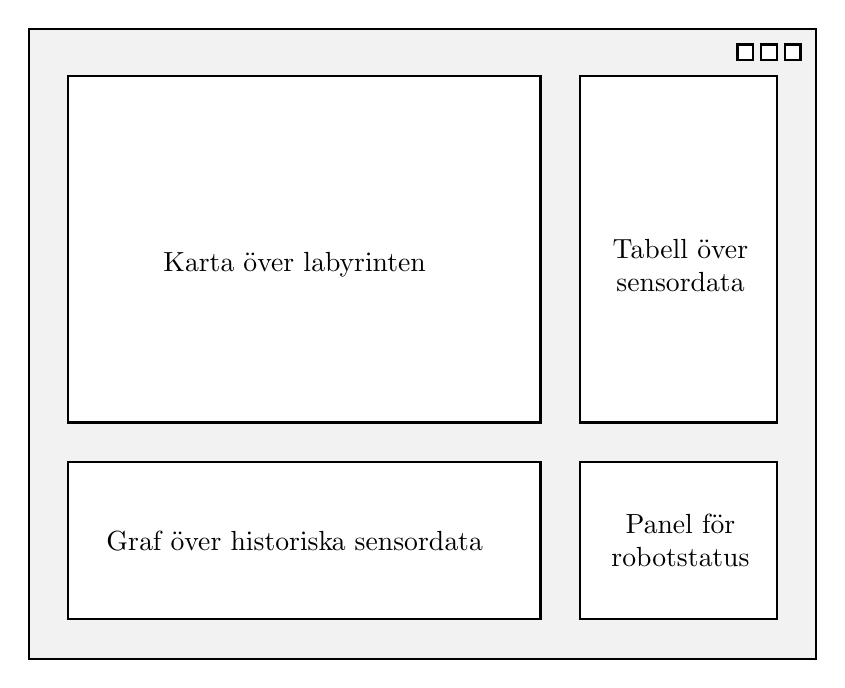
\begin{tikzpicture}[scale=1,rotate=0]
		
	%Frame
	\draw[thick, draw=black, fill=gray!10] (0,0) rectangle (10,8);

	%Exit and minimize
	\draw[thick, draw=black, fill=white] (9.0,7.6) rectangle (9.2,7.8);
	\draw[thick, draw=black, fill=white] (9.3,7.6) rectangle (9.5,7.8);
	\draw[thick, draw=black, fill=white] (9.6,7.6) rectangle (9.8,7.8);
	
	%Map
	\draw[thick, draw=black, fill=white] (0.5,3) rectangle (6.5,7.4);
	\draw  node[left, align=center, text width=5cm] at (6,5) {Karta över labyrinten};
	
	%Table
	\draw[thick, draw=black, fill=white] (7, 3) rectangle (9.5,7.4);
	\draw  node[left, align=center, text width=2cm] at (9.4,5) {Tabell över sensordata};
	
	
	%Graph
	\draw[thick, draw=black, fill=white] (0.5,0.5) rectangle (6.5,2.5);
	\draw  node[left, align=center, text width=5cm] at (6,1.5) {Graf över \mbox{historiska} sensordata};
	
	%Buttons
	\draw[thick, draw=black, fill=white] (7,0.5) rectangle (9.5,2.5);
	\draw  node[left, align=center, text width=2cm] at (9.4,1.5) {Panel för robotstatus};
	
	
	\end{tikzpicture}
	
\end{document}}
	\caption{Skiss över programvarans grafiska användargränssnitt\label{software}}	
\end{figure}

\subsubsection{Controller}
``Controller''-delen av programmet består av fyra olika klasser: ActionHandler, Handler, KeyHandler och SerialCommunicationsHandler. 
ActionHandler-klassen innehåller alla de Actions som används av programmet, det vill säga alla det metoder som anropas bland annat vid knapptryckningar.
Handler-klassen sköter samordningen av alla klasser och även programmets uppstart och instansieringen av de olika delarna.
KeyHandler-klassen sköter alla tangentbordsanrop.
SerialCommunicationsHandler-klassen sköter kommunikationen med roboten. Det innebär uppkoppling, sändning och mottagande av data samt nedkoppling av avslutning av kommunikationen. Detta sker med det publika biblioteket jSSC 2.8.0 tillsammans med datorns egna operativsystem för parning med FireFly-enheten.

\pagebreak

\section{Intermodulär kommunikation}
I denna del förklaras hur kommunikationen mellan robotens olika moduler fungerar.

\subsection{Informationsflöde}
Eftersom flera olika typer av data skickas mellan de olika modulerna inleds kommunikationen med ett ID som betecknar vilken typ av data som skickas. Dessa ID:n har värden mellan 251-255, för att kunna skiljas från alla andra värden som skickas. Andra värden än kommunikations-ID får alltså \emph{inte} anta värden större än 250. Denna uppdelning har gjorts för att underlätta felhantering.

\begin{longtable}[l]{| l | l |} \hline
\textbf{ID} & \textbf{Datatyp} \\ \hline 
255 & Styrkommando \\ \hline
254 & Kartinformation \\ \hline
253 & Sensordata \\ \hline
252 & Styrinställning \\ \hline

\caption{Tabell över kommunikations-ID}\label{kommunikationstab}
\end{longtable}

I figur \ref{informationFlow} visualiseras informationsflödet. Där anges mottagare och sändare samt vilken typ av information som går mellan dem.

\begin{figure}[htbp]
\centering
\noindent\resizebox{1\linewidth}{!}{
	\documentclass[border=10px]{standalone}
\usepackage{tikz}
\usetikzlibrary{patterns}
\usetikzlibrary{shapes.geometric}
\usetikzlibrary{shapes.arrows}
\usepackage{amssymb}
\usetikzlibrary{calc}
\usepackage{verbatim}

\pagestyle{empty}
\begin{document}

\tikzstyle{decision} = [diamond, draw,
    text width=4em, text badly centered, node distance=3cm, inner sep=0pt]
    
\tikzstyle{block} = [rectangle, draw,
    text width=7em, text centered, rounded corners, minimum height=4em]
	
\begin{tikzpicture}[scale=1]

%http://www.texample.net/tikz/examples/simple-flow-chart/

\node (robot) at (-1,4.2) {\verb+Robot+};
\node[block] (styr) at (0,0) {Styrmodul};
\node[block] (sensor) at (3.5,3) {Sensormodul};
\node[block] (huvud) at (7,0) {Huvudmodul};
\draw[dashed] (-1.65,-2) rectangle (8.6,4);

\node[block] (dator) at (15,0) {Datormodul};


\draw[-latex, bend left] (huvud) edge node[above]{Kartinformation} node[below]{Sensordata}(dator);
\draw[-latex, bend left] (dator) edge node[below]{Styrkommandon} node[above]{Styrinställningar} (huvud);

\draw[-latex, bend left] (huvud) edge node[below]{Sensordata}(styr);
\draw[-latex] (huvud) edge node[above]{Styrkommandon} (styr);
\draw[-latex, bend right] (huvud) edge node[above]{Styrinställningar} (styr);

\draw[->] (sensor.east) -| node[above]{Sensordata}(huvud.north);
	\end{tikzpicture}
	
\end{document}}
	\caption{Schema över informationsflödet\label{informationFlow}}	
\end{figure}

\subsubsection{Kommunikationsprotokoll - styrkommandon}
Protokollet som används för att skicka styrkommandon både datormodul $\rightarrow$ huvudmodul och huvudmodul $\rightarrow$ styrmodul finns illustrerat i figur \ref{styrdata}.

\begin{figure}[htbp]
\centering
\noindent\resizebox{.8\linewidth}{!}{
	\documentclass[crop,tikz]{standalone}
\usepackage{tikz}
\usetikzlibrary{calc}
\usetikzlibrary{positioning}
\begin{document}
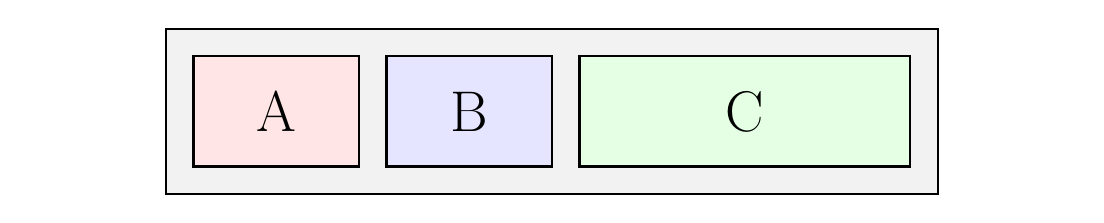
\begin{tikzpicture}[scale=0.07,rotate=0]
	
	%Background
	\draw[draw=white, fill=white] (0,0) rectangle (190,30);
		
	%Frame
	\draw[thick, draw=black, fill=gray!10] (25,0) rectangle (165,30);

	%Segments
	%A
	\draw[thick, draw=black, fill=red!10] (30,5) rectangle (60,25);
	\node at (45,15) {\huge A};

	%B
	\draw[thick, draw=black, fill=blue!10] (65,5) rectangle (95,25);
	\node at (80,15) {\huge B};
	
	%C
	\draw[thick, draw=black, fill=green!10] (100,5) rectangle (160,25);
	\node at (130,15) {\huge C};
	

	
\end{tikzpicture}
\end{document}}
	\caption{Protokoll för överföring av styrkommandon\label{styrdata}}	
\end{figure}

Respektive segment motsvarar följande: 
\begin{itemize}
	\item A (1 byte) - Kommunikations-ID, se tabell \ref{kommunikationstab}.
	\item B (1 byte) - Definierar vilket kommando som skickas, se tabell \ref{styrtab}.
	\item C (1 byte) - Hastighet om manuellt läge, valfritt i autonomnt då det inte tas hänsyn till (tillåtna värden: 0-245).
\end{itemize}

\subsubsection{Kommunikationsprotokoll - kartinformation}
Huvudmodulen kommer för varje ny kartmodul skicka data till datormodulen som ritar upp den nya informationen grafiskt. Varje kartmodul representeras av en position i en tvådimensionell array. För överföring av denna information används följande protokoll:

 \begin{figure}[H]
\centering
\noindent\resizebox{.8\linewidth}{!}{
	\documentclass[crop,tikz]{standalone}
\usepackage{tikz}
\usetikzlibrary{calc}
\usetikzlibrary{positioning}
\begin{document}
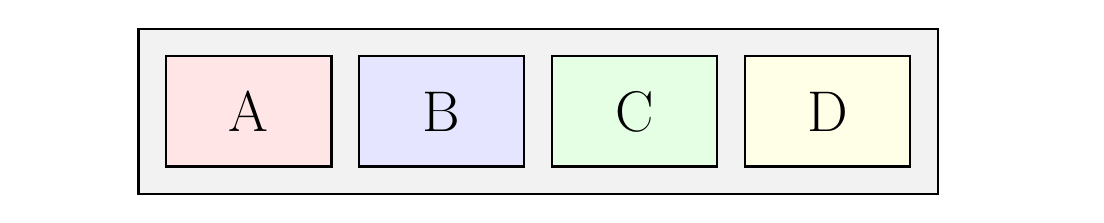
\begin{tikzpicture}[scale=0.07,rotate=0]
		
	%Background
	\draw[draw=white, fill=white] (0,0) rectangle (190,30);	
		
	%Frame
	\draw[thick, draw=black, fill=gray!10] (20,0) rectangle (165,30);

	%Segments
	%A
	\draw[thick, draw=black, fill=red!10] (25,5) rectangle (55,25);
	\node at (40,15) {\huge A};

	%B
	\draw[thick, draw=black, fill=blue!10] (60,5) rectangle (90,25);
	\node at (75,15) {\huge B};
	
	%C
	\draw[thick, draw=black, fill=green!10] (95,5) rectangle (125,25);
	\node at (110,15) {\huge C};
	
	%D
	\draw[thick, draw=black, fill=yellow!10] (130,5) rectangle (160,25);
	\node at (145,15) {\huge D};
	
\end{tikzpicture}
\end{document}}
	\caption{Protokoll för överföring av kartdata \label{kartdata}}	
\end{figure} 

Respektive segment motsvarar följande: 
\begin{itemize}
	\item A (1 byte) - Kommunikations-ID, se tabell \ref{kommunikationstab}.
	\item B (1 byte) - x-koordinat (tillåtna värden: 0-28).
	\item C (1 byte) - y-koordinat (tillåtna värden: 0-28).
	\item D (1 byte) - Information om vad som finns i noden, se tabell \ref{maptab}.
\end{itemize}

\subsubsection{Kommunikationsprotokoll - sensordata}
Sensordata skickas enligt protokollet i figur \ref{sensordata}.

 \begin{figure}[H]
\centering
\noindent\resizebox{.8\linewidth}{!}{
	\documentclass[crop,tikz]{standalone}
\usepackage{tikz}
\usetikzlibrary{calc}
\usetikzlibrary{positioning}
\begin{document}
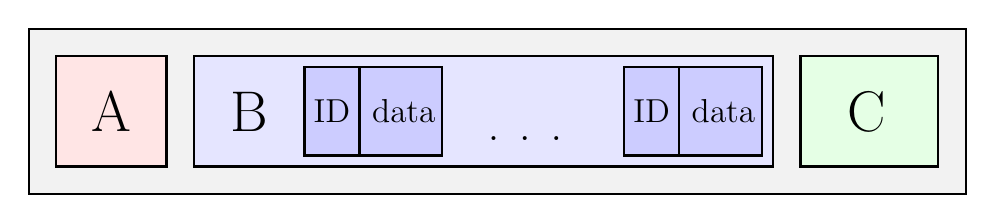
\begin{tikzpicture}[scale=0.07,rotate=0]
		
	%Frame
	\draw[thick, draw=black, fill=gray!10] (0,0) rectangle (170,30);

	%Segments
	%A
	\draw[thick, draw=black, fill=red!10] (5,5) rectangle (25,25);
	\node at (15,15) {\huge A};

	%B
	\draw[thick, draw=black, fill=blue!10] (30,5) rectangle (135,25);
	\node at (40,15) {\huge B};
	
	%B1
	\draw[thick, draw=black, fill=blue!20] (50,7) rectangle (60,23);
	\draw[thick, draw=black, fill=blue!20] (60,7) rectangle (75,23);
	\node at (55,15) {\large ID};
	\node at (68,15) {\large data};
	
	\node at (90,10) {\LARGE . . .};
	
	%Bn
	\draw[thick, draw=black, fill=blue!20] (118,7) rectangle (133,23);
	\draw[thick, draw=black, fill=blue!20] (108,7) rectangle (118,23);
	\node at (113,15) {\large ID};
	\node at (126,15) {\large data};

	%C
	\draw[thick, draw=black, fill=green!10] (140,5) rectangle (165,25);
	\node at (152,15) {\huge C};
	
\end{tikzpicture}
\end{document}}
	\caption{Protokoll för överföring av sensordata\label{sensordata}}	
\end{figure} 

Respektive segment motsvarar följande: 
\begin{itemize}
	\item A - Kommunikations-ID, se tabell \ref{kommunikationstab}.
	\item B - Sensordatapaket
	\begin{itemize}
	\item ID (1 byte) - identifierar sensorn, se tabell \ref{sensortab}.
	\item Data (1 byte) - sensorns värde (tillåtna värden: 0-245).
	\end{itemize}
\end{itemize}

\subsubsection{Kommunikationsprotokoll - styrinställningar}
Protokollet som används för att skicka styrinställningar både datormodul $\rightarrow$ huvudmodul och huvudmodul $\rightarrow$ styrmodul finns illustrerat i figur \ref{styrkomm}.

\begin{figure}[htbp]
\centering
\noindent\resizebox{.8\linewidth}{!}{
	\documentclass[crop,tikz]{standalone}
\usepackage{tikz}
\usetikzlibrary{calc}
\usetikzlibrary{positioning}
\begin{document}
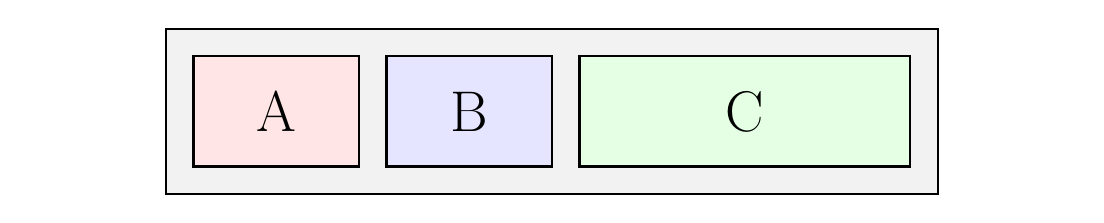
\begin{tikzpicture}[scale=0.07,rotate=0]
	
	%Background
	\draw[draw=white, fill=white] (0,0) rectangle (190,30);
		
	%Frame
	\draw[thick, draw=black, fill=gray!10] (25,0) rectangle (165,30);

	%Segments
	%A
	\draw[thick, draw=black, fill=red!10] (30,5) rectangle (60,25);
	\node at (45,15) {\huge A};

	%B
	\draw[thick, draw=black, fill=blue!10] (65,5) rectangle (95,25);
	\node at (80,15) {\huge B};
	
	%C
	\draw[thick, draw=black, fill=green!10] (100,5) rectangle (160,25);
	\node at (130,15) {\huge C};
	

	
\end{tikzpicture}
\end{document}}
	\caption{Protokoll för överföring av styrkommandon\label{styrkomm}}	
\end{figure}

Respektive segment motsvarar följande: 
\begin{itemize}
	\item A (1 byte) - Kommunikations-ID, se tabell \ref{kommunikationstab}.
	\item B (1 byte) - Definierar vilken styrinställning som skickas, se tabell \ref{styrinsttab}.
	\item C (4 byte) - 0/1 om av/på, annars flyttal (C float).
\end{itemize}

\subsection{Tabeller}

\begin{longtable}[l]{| l | l |} \hline
\textbf{ID} & \textbf{Kartinformation} \\ \hline 
244 & Vägg \\ \hline
243 & Mål \\ \hline
242 & Start \\ \hline
[0,225] & Där roboten åkt \\ \hline

\caption{Tabell över kartvärden }\label{maptab}
\end{longtable}

\begin{longtable}[l]{| l | l | c |} \hline
\textbf{ID} & \textbf{Sensor} & \textbf{Enhet} \\ \hline 
1 & IR-sensor höger-fram & cm \\ \hline
2 & IR-sensor vänster-fram  & cm \\ \hline
3 & IR-sensor höger-bak  & cm  \\ \hline
4 & IR-sensor vänster-bak  &  cm \\ \hline
5 & Lasersensor (high) & cm  \\ \hline
6 & Lasersensor (low) & cm  \\ \hline
7 & Rotation kring z-axeln & rad/s \\ \hline
8 & IR-sensor för mål & 0/1 \\ \hline
\caption{Tabell över sensorerna}\label{sensortab}
\end{longtable}

\begin{longtable}[l]{| l | l |} \hline
\textbf{ID} & \textbf{Styrkommando} \\ \hline 
1 & Kör fram \\ \hline
2 & Kör bak \\ \hline
3 & Rotera åt höger \\ \hline
4 & Rotera åt vänster \\ \hline
5 & Fram och höger \\ \hline
6 & Fram och vänster \\ \hline
7 & Bak och höger \\ \hline
8 & Bak och vänster \\ \hline
9 & Gripklo öppna/stäng \\ \hline

\caption{Tabell över styrkommandon}\label{styrtab}
\end{longtable}

\begin{longtable}[l]{| l | l |} \hline
\textbf{ID} & \textbf{Styrinställning} \\ \hline 
1 & Reglering av/på \\ \hline
2 & P-värde \\ \hline
3 & D-värde \\ \hline
4 & K-värde \\ \hline

\caption{Tabell över styrinställningar}\label{styrinsttab}
\end{longtable}


\begin{table}[h]
\begin{tabular}{|l|l|l|l|l|} \hline

\textbf{Kommando} & \textbf{Id} & \textbf{Info} & \textbf{Kommentar}\\ \hline

252 & 1 & 1/0 & 1 om reglering är på, 0 annars \\ \hline
252 & 2 & Data & Regleringfunktionens P-värde \\ \hline
252 & 3 & Data & Regleringfunktionens D-värde \\ \hline
252 & 4 & 1/0 & 1 om gripklo ska vara öppen, 0 om den ska vara stängd \\ \hline


253 & 1 & 1 & Data för främre högra IR-sensorn kommer skickas härnäst \\ \hline
253 & 2 & Data & Värde på den främre högra IR-sensorn \\ \hline
253 & 3 & 2 & Data för främre vänstra IR-sensorn kommer skickas härnäst \\ \hline
253 & 4 & Data & Värde på den främre vänstra IR-sensorn \\ \hline
253 & 5 & 3 & Data för bakre högra IR-sensorn kommer skickas härnäst \\ \hline
253 & 6 & Data & Värde på den bakre högra IR-sensorn \\ \hline
253 & 7 & 4 & Data för bakre vänstra IR-sensorn kommer skickas härnäst \\ \hline
253 & 8 & Data & Värde på den bakre vänstra IR-sensorn \\ \hline

253 & 9 & 5 & LIDAR-Lite's 8 mest signifikanta bitar kommer skickas härnäst \\ \hline
253 & 10 & Data & Värde på LIDAR-Lite's 8 mest signifikanta bitar \\ \hline
253 & 11 & 6 & LIDAR-Lite's 8 minst signifikanta bitar kommer skickas härnäst \\ \hline
253 & 12 & Data & Värde på LIDAR-Lite's 8 minst signifikanta bitar \\ \hline

253 & 13 & 7 & Data för gyrot kommer skickas härnäst \\ \hline
253 & 14 & Data & Värde på gyrot \\ \hline

253 & 15 & 8 & Data för IR-detektorn kommer skickas härnäst \\ \hline
253 & 16 & 1/0 & 1 skickas om målet är upptäckt, 0 annars \\ \hline

255 & - & - & Kommando att köra framåt \\ \hline
255 & - & Data/not care\text{*} & Hur fort roboten ska köras framåt \\ \hline
255 & - & - & Kommando att köra bakåt \\ \hline
255 & - & Data/not care & Hur fort roboten ska köras bekåt \\ \hline
255 & - & - & Kommando att rotera höger \\ \hline
255 & - & Data/not care & Hur fort roboten ska rotera åt höger  \\ \hline
255 & - & - & Kommando att rotera vänster \\ \hline
255 & - & Data/not care & Hur fort roboten ska rotera åt vänster  \\ \hline

\end{tabular}
\end{table}

\text{*} Reagerar på data vid manuellt läge och ignorerar data vid autonomt

\section{Slutsatser}
\textit{Vilka förbättringar skulle kunna göras?}

\pagebreak
\addcontentsline{toc}{section}{Referenser}
\bibliographystyle{ieeetr}
\bibliography{references}

\pagebreak


\appendix

\end{flushleft}

\end{document}

